\chapter{Resultados} \label{resultado}

Para a primeira etapa do projeto, fizemos a análise do erro e discrepância para os dados de São Paulo. Por problemas na aplicação que coleta as geocodificações, obtivemos resultados apenas para 3 APIs (TomTom, Mapbox e Here). Abaixo serão apresentados os resultados obtidos.

\section{Distribuição Espacial dos Pontos Geocodificados}

Após a geocodificação dos dados, tornou-se interessante visualizar como os pontos geocodificados estavam distribuídos no espaço e quão diferentes eram em relação aos pontos de referência ("Gold"). Para essa finalidade, foram gerados mapas identificando os pontos para cada uma das APIs.

É importante observar que, com base apenas nessa visualização, não é possível tirar conclusões definitivas. No entanto, é possível analisar a densidade dos pontos e identificar que, em todas as APIs, houve uma maior concentração de dados "Gold". No entanto, em algumas APIs, essa concentração é visivelmente menor do que em outras. Além disso, é notável que os pontos classificados como "Gold" estão concentrados na região metropolitana de São Paulo, enquanto alguns pontos geocodificados estão localizados fora dessa região, em outras cidades do estado. Essa disparidade provavelmente reflete a ocorrência de alguns erros graves de geocodificação, conhecidos como "outliers".

Na Figura \ref{fig:mapapontos1}, podemos visualizar a distribuição espacial dos pontos geocodificados pela Mapbox. Nela, é possível observar a presença dos outliers mencionados anteriormente. No entanto, é importante ressaltar que esses casos de erro são relativamente raros. Portanto, considerando apenas essa análise, a API obteve resultados satisfatórios.

\begin{figure}[h] 
  \centering
  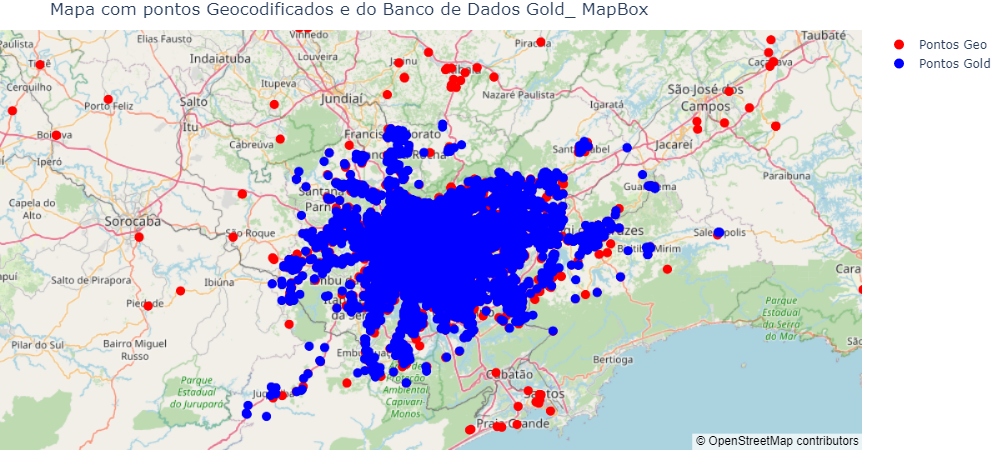
\includegraphics[width=0.8\textwidth]{Figuras/mapapontos1.png}
  \caption{Mapa da Distribuição Espacial dos Pontos da base Gold e Geocodificados pela Mapbox}
  \label{fig:mapapontos1}
\end{figure}

Na Figura \ref{fig:mapapontos2}, podemos observar a distribuição espacial dos pontos geocodificados pela Here. Fica claro na imagem que houve uma diminuição significativa dos pontos, indicando uma baixa resposta da API. Com essa quantidade reduzida de pontos, não é possível tirar conclusões sólidas sobre os dados. No entanto, é evidente que, além da baixa resposta, os pontos parecem estar dispersos em locais distintos. Esses resultados foram considerados insatisfatórios. Em um momento subsequente, o experimento será repetido para que possamos obter conclusões mais precisas.

\begin{figure}[h]
  \centering
  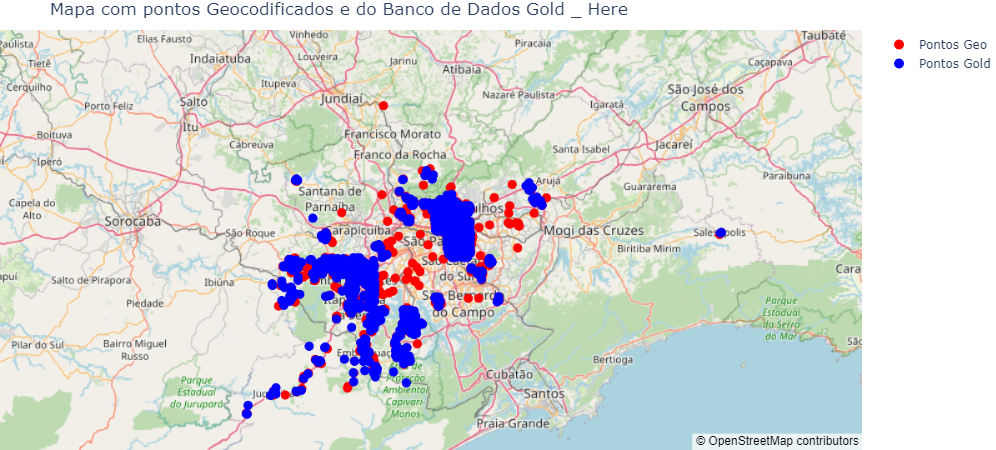
\includegraphics[width=0.8\textwidth]{Figuras/mapapontos2.png}
  \caption{Mapa da Distribuição Espacial dos Pontos da base Gold e Geocodificados pela Here}
  \label{fig:mapapontos2}
\end{figure}

Já a Figura \ref{fig:mapapontos3} mostra a distribuição espacial dos pontos geocodificados pela TomTom. Com esse mapa, é possível observar que a resposta da API foi boa em comparação com os mapas apresentados anteriormente. Embora ainda tenha alguns "outliers", aparentemente esses estão em maior quantidade do que na Figura \ref{fig:mapapontos3} e estão mais dispersos geograficamente. No entanto, considerando apenas essa análise, o resultado é considerado satisfatório.

\begin{figure}[h]
  \centering
  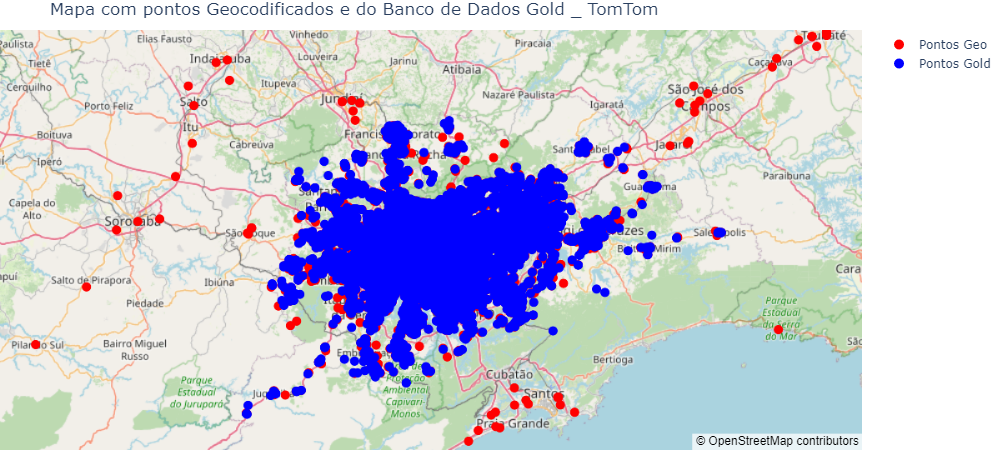
\includegraphics[width=0.8\textwidth]{Figuras/mapapontos3.png}
  \caption{Mapa da Distribuição Espacial dos Pontos da base Gold e Geocodificados pela TomTom}
  \label{fig:mapapontos3}
\end{figure}



\section{Metrícas do Erro}
A próxima etapa foi o calculo do erro para cada um dos pontos, sendo este expresso em quilômetros (Km).

Com o erro de cada um dos pontos, foram calculadas as métricas mencionadas anteriormente. A \ref{tab:tabelaDeMetricas} mostra esses resultados.

Em relação a taxa de resposta, ou seja, a quantidade de endereços que foram geocodificados, a TomTom tem o melhor resultado, com um índice superior a 80\%, seguida pela Mapbox, com taxa de 53,38\%. A Here obteve uma taxa de resposta baixa, como esperado pela análises anteriores. Apesar de ter uma API com taxa de resposta alta, esse resultado foi considerado limitante para equipe pois nos impede de fazer algumas análises.
Outra métrica importante é a taxa de acerto. Foi considerado como acerto aqueles endereços que tiveram erro menor que 150m (0.015Km). A taxa de acerto foi baixíssima para todas as APIs, sendo a melhor 30.19\%. Esse é um resultado péssimo para os dados acumulados. Porém, devido a baixa quantidade de dados não é possível concluir que as APIs em questão tem uma performance ruim. Na próxima etapa do projeto iremos fazer a análise comparativa dos resultados com as outras APIs e com uma maior quantidade de dados. 

Outras métricas interessantes obtidas foram as métricas de média, mediana e desvio padrão. Com elas é possível ver o comportamento geral do erro em cada uma das APIs. As médias foram muito altas, indo de 2Km a 10Km. O desvio padrão também foi alto, mostrando que há uma grande veriação no erro. Apesar disso, a mediana foi bem baixa, alcançando resultados desejáveis na nossa pesquisa. A média aparada obteve resultados muito bons, o que indica que com a retirada dos outliers as métricas tendem a melhorar. Como trabalho futuro, pretendemos refazer as análises com o corte em 50km de erro. De forma geral, esses resultados foram considerados insatisfatórios. Ao longo do relatório, iremos analisar outras questões em detalhes.

\begin{table}
  \centering
  \caption{Métricas de Erro e Resposta}
  \label{tab:tabelaDeMetricas}
  \setlength{\tabcolsep}{4pt}
  \begin{tabular}{|c|c|c|c|c|c|c|}
  \hline
  \makecell{API} & \makecell{Média \\(km)} & \makecell{Mediana \\(km)} & \makecell{Desvio \\Padrão (km)} & \makecell{Média \\Aparada (km)} & \makecell{Taxa de \\Resposta (\%)} & \makecell{Taxa de \\Acerto(\%)}\\
  \hline
  Mapbox & 9.7544 & 0.1084 & 46.7664 & 1.8349 & 53.3829 & 30.1903 \\
  Tomtom & 5.0701 & 0.0560 & 35.6215 & 0.2373 & 83.1894 & 9.2051 \\
  Here & 2.2372 & 0.0632 & 13.7984 & 0.4365 & 13.9075 & 9.2051 \\
  \hline
  \end{tabular}
\end{table}

\section{Distribuição do Erro}

Em seguida, foi realizada a análise da distribuição do erro para cada uma das GeoAPIs. 

Para isso, utilizamos histogramas de erro individualmente para cada API e combinando todas elas. Na \ref{fig:hist-global} é mostrado os histogramas para cada uma das APIs e o histograma que é a combinação de todas elas. No entanto, devido à presença de alguns erros exorbitantes, esses histogramas não são muito representativos, pois a maior parte do erro se concentrava entre 0 km e 50 km. Esse intervalo é considerado um erro muito grande, o que dificulta a obtenção de conclusões sólidas.

\begin{figure}[ht]
  \centering
  \begin{subfigure}[b]{0.45\textwidth}
    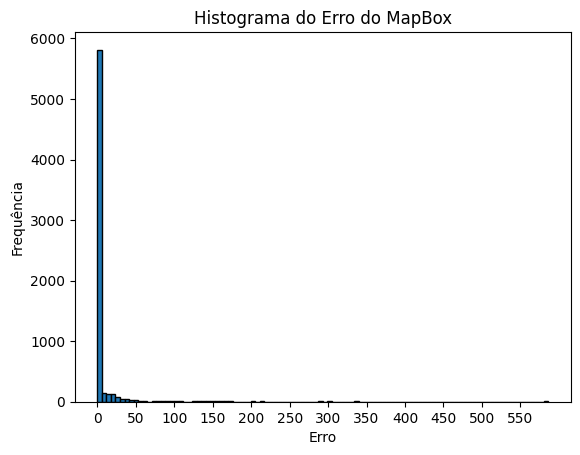
\includegraphics[width=\textwidth]{Figuras/hist1.png}
    \caption{Mapbox}
    \label{fig:hist1}
  \end{subfigure}
  \hfill
  \begin{subfigure}[b]{0.45\textwidth}
    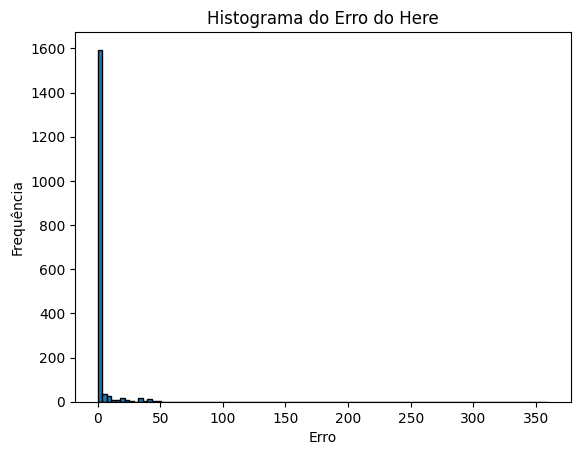
\includegraphics[width=\textwidth]{Figuras/hist2.png}
    \caption{Here}
    \label{fig:hist2}
  \end{subfigure}

  \begin{subfigure}[b]{0.45\textwidth}
    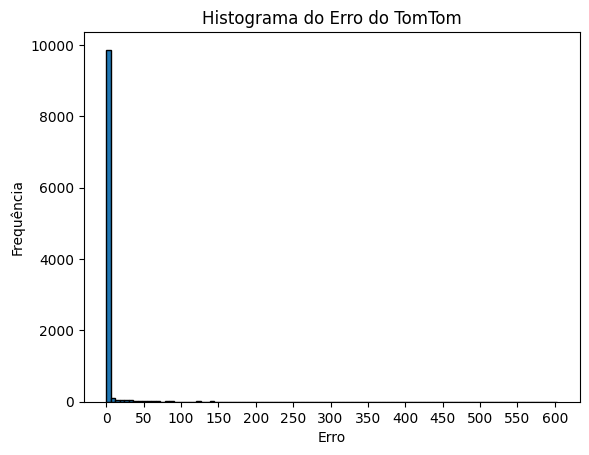
\includegraphics[width=\textwidth]{Figuras/hist3.png}
    \caption{TomTom}
    \label{fig:hist3}
  \end{subfigure}
  \hfill
  \begin{subfigure}[b]{0.45\textwidth}
    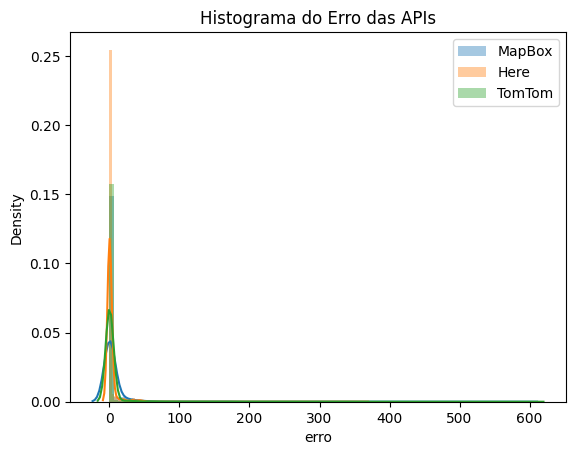
\includegraphics[width=\textwidth]{Figuras/hist4.png}
    \caption{Comparativo entre as APIs}
    \label{fig:hist4}
  \end{subfigure}
  
  \caption{Histogramas do erro das 3 APIs para o todos os dados.}
  \label{fig:hist-global}
\end{figure}

Diante disso, decidimos realizar um corte nos dados, limitando o erro em 0,5 km ou 500 metros. Em seguida, repetimos o processo, gerando agora um único histograma que representa a distribuição do erro para todas as APIs em conjunto. A Figura \ref{fig:histLimitado} apresenta esse histograma. Nele, observamos que a maior parte dos dados está concentrada entre erros de 0,0 km e 0,1 km. Isso confirma a hipótese de que as métricas se comportariam melhor com a remoção dos outliers.

Em relação às APIs, nessa faixa de erro, a TomTom apresenta um desempenho superior, com uma curva mais estreita e mais próxima de 0. No entanto, a diferença entre as APIs não é significativa.

 
\begin{figure}[h]
  \centering
  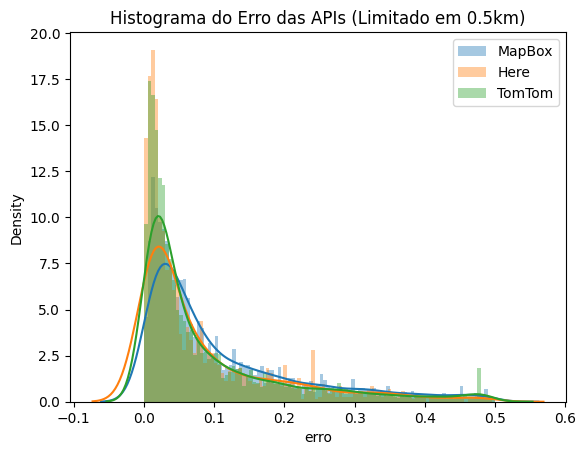
\includegraphics[width=0.8\textwidth]{Figuras/hist5.png}
  \caption{Histograma comparativo do erro das APIs limitado em 500 metros}
  \label{fig:histLimitado}
\end{figure}

De forma geral, embora o histograma seja uma ferramenta poderosa para a análise da distribuição do erro, neste caso, ele não se mostrou tão eficiente devido às limitações decorrentes da presença de valores excessivamente altos.


\section{Distribuição Espacial do Erro}

Além disso, realizamos uma análise adicional para visualizar como esse erro se comporta no espaço. Para isso, criamos mapas de altitude, onde o erro foi utilizado como medida de altitude. O mapa consiste em linhas de altitude, criadas a partir da interpolação do erro dos pontos. Em seguida essas linhas foram transformadas em um polígono e coloridas de acordo com os valores de altitude. Nessa representação, cores mais próximas do vermelho indicam erros mais altos, enquanto cores mais próximas do azul escuro indicam erros mais baixos. Também plotamos os pontos geocodificados no mapa para avaliar a representatividade das cores. Dessa forma, pudemos verificar se uma determinada área apresenta muitos pontos geocodificados ou se há poucos pontos com erros grandes. Todo esse processo foi realizado utilizando as bibliotecas do python matplotlib, scipy e folium para a criação e vizualização do gráficos; e as biblicotecas pandas e numpy para manipulação de estruturas de dados utilizadas. 

Ao analisar os resultados, observamos que a maioria do mapa apresenta erros menores que 34 km, conforme observado nos histogramas acima. No entanto, identificamos alguns pontos com erros grandes, que serão avaliados individualmente posteriormente. É importante ressaltar que encontramos uma limitação devido à presença de erros exorbitantes, ou outliers, o que restringe nossa capacidade de tirar conclusões significativas. Para obter uma melhor compreensão do contraste e da distribuição geográfica do erro, planejamos repetir o experimento realizando um corte em 34 km.

É válido destacar que o mapa é interativo no projeto original, permitindo uma visualização mais detalhada das informações apresentadas.

Na \ref{fig:grafAltM} conseguimos ver a abrangência da geocodificação da Mapbox, ou seja, os pontos geocodificados conseguiram abranger boa parte da região metropolitana de São Paulo. Além disso, o erro ficou concentrado em 25 Km na maior parte do gráfico. Em alguns pontos ela apresentou erros ente 50 km e 100 km, o que já é considerado um ponto preocupante. Existiram alguns erros na faixa de 300 km nas periferias da cidade. Porém, se pode observar que há uma baixíma concentração de pontos, o que indica que existem poucos pontos com erro baixo, que causaram essa vizualização. No centro, existem alguns pontos avermelhados que possuem uma grande concentração de pontos, esse é um dado preocupante pois indica que a API realmente está errando bastante em relação aos dados referência naquela região.

\begin{figure}[h] 
  \centering
  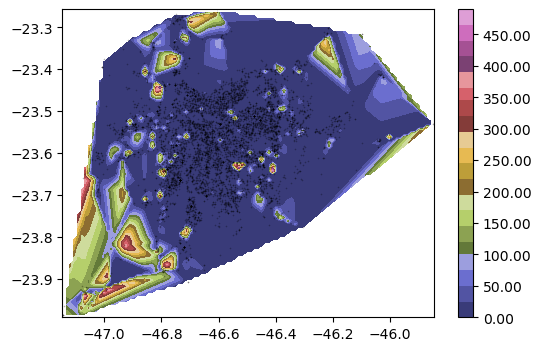
\includegraphics[width=0.8\textwidth]{Figuras/graficoAltPontosMapbox.png}
  \caption{Gráfico de altitude do erro (km) da geocodificação da Mapbox.}
  \label{fig:grafAltM}
\end{figure}

Já a \ref{fig:grafAltH} demostra a baixa abrangência da geocodificação da Here. Como apresentado anteriormente, essa GeoAPI teve a menor texa de resposta e a vizualização pelo gráfico de altitude só confirma isso. Sendo assim, qualquer análise realizada será inviesada. É possível observar uma grande concentração de azul, ou seja, os dados tem erro pequeno. Tem alguns picos, com erro elevado, porém somente um apresenta pontos suficientes para considerar que a região tem erro alto. 

\begin{figure}[h]
  \centering
  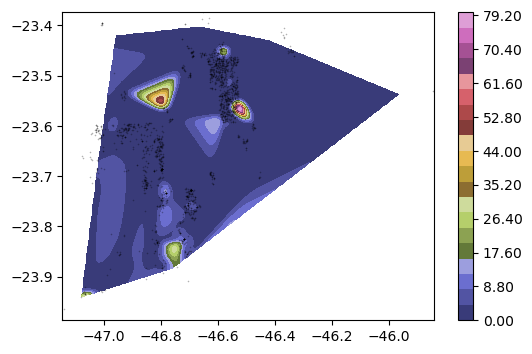
\includegraphics[width=0.8\textwidth]{Figuras/graficoAltPontosHere.png}
  \caption{Gráfico de altitude do erro (km) da geocodificação da Here.}
  \label{fig:grafAltH}
\end{figure}

A \ref{fig:grafAltT} mostra é similar a \ref{fig:grafAltM} pois também teve uma taxa de resposta suficientemente grande. A maior parte do gráfico possui uma cor azul escura, o que indica que o erro nessas regiões é menor que 20 km. Porém possui alguns picos escverdeados que mostram um erro bem alto. Em alguns deles não é possível observar uma grande concentração de pontos, o que indica que são poucos pontos com erro grandes. Já no centro da figura, onde há grande concentração de pontos, esses picos também aparecem, o que indica um erro alto nessa região.
\begin{figure}[h]
  \centering
  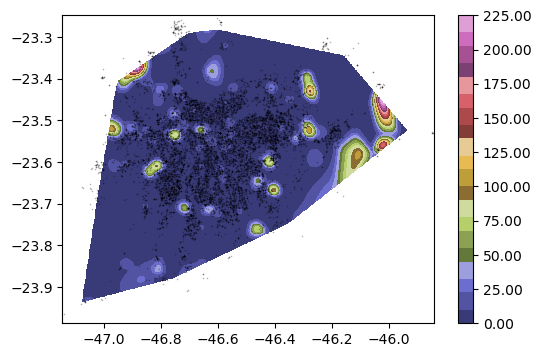
\includegraphics[width=0.8\textwidth]{Figuras/graficoAltPontosTomtom.png}
  \caption{Gráfico de altitude do erro (km) da geocodificação da TomTom.}
  \label{fig:grafAltT}
\end{figure}

\section{Relações entre erro e discrepância}
Por fim, foi realizada a análise comparativa entre erro e discrepância. A medida escolhida para essa análise foi a covariância. Calculamos a covariância entre a latitude e a longitude para cada ponto utilizando as 3 APIs e depois foi calculada a média das duas covariâncias citadas anteriormente. Foram considerados para análise apenas os pontos em que se tem informação das 3 APIs. Devido ao fato da API Here ter tido uma taxa de resposta tão baixa, a quantidade de pontos obtidas foi também muito baixa.Fizemos então uma análise com apenas 1683 endereços da base. 

Após o calculo da covariância, construímos para cada uma das APIs um gráfico de covariância pelo erro referente. Nos gráficos das figuras \ref{fig:CovErroM} e \ref{fig:CovErroT} não é possível observar uma relação entre as duas medidas. O primeiro mostra que os valores de erro estão concentrados na faixa de 0km a 50km para esses dados. No segundo gráfico há uma variação maior do erro, mas essa variação não reflete na variação da da covariância. Os dados indicam que essa relação não existe, porém não é possível tiral tal conclusão devido a quantidade baixa de dados. 

\begin{figure}[h]
  \centering
  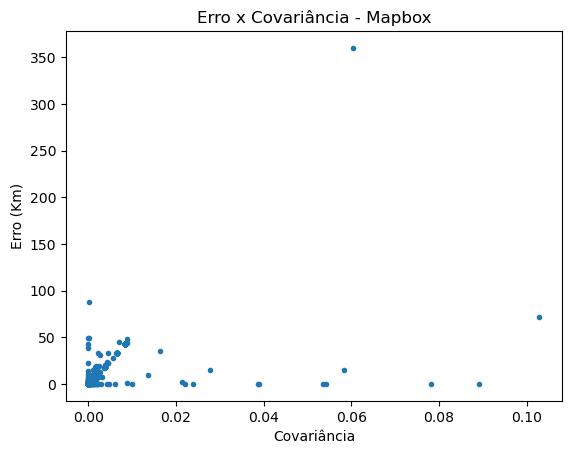
\includegraphics[width=0.8\textwidth]{Figuras/ErroCovM.png}
  \caption{Gráfico covariância por erro da Mapbox}
  \label{fig:CovErroM}
\end{figure}

\begin{figure}[h]
  \centering
  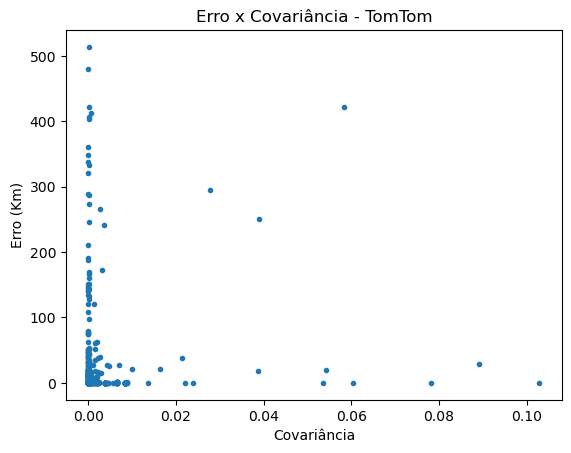
\includegraphics[width=0.8\textwidth]{Figuras/ErroCovT.png}
  \caption{Gráfico covariância por erro da TomTom}
  \label{fig:CovErroT}
\end{figure}

A \ref{fig:CovErroH} apresenta resultados diferentes dos anteriores. No gráfico pode-se ver uma relação próxima a linear, onde a medida que o erro cresce, a covariância cresce junto. Como os dados de covariância estão concentrados em 0 a 0.02 e os dados de erro em 0km a 100km, as faixas apresentam mais pontos. É um resultado promissor, porém devem ser feitas mais análises devido a quantidade de dados. 

\begin{figure}[h]
  \centering
  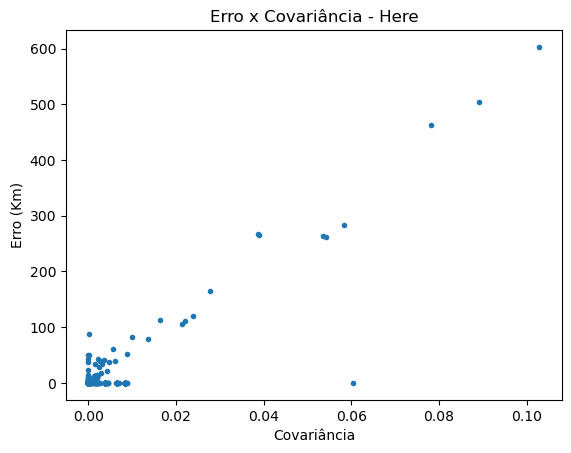
\includegraphics[width=0.8\textwidth]{Figuras/ErroCovH.png}
  \caption{Gráfico covariância por erro da Here}
  \label{fig:CovErroH}
\end{figure}
